\section{含参积分}
\label{sec:integ-parametric}

很多量由一个依赖参数的积分给出，例如$F(t)=\int_0^\infty e^{-tx}\,\mathrm dx$，或下一章的局部平均$\int\rho_\varepsilon(x-y)f(y)\,\mathrm dy$。我们关心$F$作为参数的函数是否连续、是否可导，导数能否移到积分号内计算。这些问题都可以化为函数列的积分极限：参数$t_n\to t$时，被积函数$f(\cdot,t_n)$构成一列函数，差商构成另一列函数。所以支配收敛定理是本节的主要工具，关键是找出合适的共同上界。先处理固定的积分区域，再讨论积分区域随参数移动时的额外变化。

\subsection{积分对参数的连续性}
\label{sec:integ-parameter-continuity}

\paragraph{连续性定理}
设$(X,\mathcal A,\mu)$是测度空间，参数$t$取值于度量空间$T$，$f:X\times T\to\mathbb C$，并且每个$f(\cdot,t)$可测。令$F(t)=\int_Xf(x,t)\,\mathrm d\mu(x)$。被积函数关于参数的逐点连续性不足以推出$F$连续，还需要一个与参数无关的可积上界，防止质量在参数变化时逃逸。

\begin{theorem}[含参积分的连续性]
\label{thm:integ-parameter-continuity}
设$t_0\in T$，$U$是$t_0$的邻域。若存在零测集$N$与可积函数$g\geq0$，使对每个$x\notin N$：
\begin{enumerate}
 \item $t\mapsto f(x,t)$在$t_0$处连续；
 \item 对一切$t\in U$，$\lvert f(x,t)\rvert\leq g(x)$，
\end{enumerate}
则$F$在$U$上有定义，并在$t_0$处连续。
\end{theorem}

\begin{proof}
由第2条，每个$f(\cdot,t)$（$t\in U$）可积，$F$在$U$上有定义。度量空间中的连续性可以用序列检验：任取$t_n\to t_0$，不妨设$t_n\in U$。函数列$f(\cdot,t_n)$在$N$外收敛到$f(\cdot,t_0)$，并由同一个$g$控制。由支配收敛定理，$F(t_n)\to F(t_0)$。
\end{proof}

定理要求的控制是对参数邻域内\emph{所有}$t$同时成立的：控制的是参数变化后的函数值，而不只是$t_0$处的函数值。零测集$N$也必须与$t$无关，因为参数可以取不可数多个值，而不可数个零测例外的并不一定零测。

例如$F(t)=\int_0^\infty e^{-x}\cos(tx)\,\mathrm dx$。对每个$x$，$t\mapsto e^{-x}\cos(tx)$连续，并且$\lvert e^{-x}\cos(tx)\rvert\leq e^{-x}$对一切$t\in\mathbb R$成立，$e^{-x}$在$[0,\infty)$上可积，所以$F$在$\mathbb R$上处处连续。

\paragraph{控制失效的情形}
在$[0,\infty)$上取$f(x,t)=te^{-tx}$，$t\geq0$。对每个固定的$x>0$，$t\mapsto te^{-tx}$连续，在$t=0$处取$0$。但$t>0$时$F(t)=\int_0^\infty te^{-tx}\,\mathrm dx=1$，而$F(0)=0$，$F$在$0$处不连续。

图~\ref{fig:integ-parameter-continuity}显示了原因：$t$越小，曲线越低、越向右摊开，面积始终为$1$；质量没有消失，而是逃向无穷远处。任何控制函数都不小于包络$\sup_{t>0}te^{-tx}=1/(ex)$（在$t=1/x$处取到），它在无穷远处不可积，所以$t=0$附近不存在可积的共同上界。与尖峰例子相比，这里质量不是挤进窄区间，而是摊到无界区域上，支配条件同样排除了这种情况。

\begin{figure}[!htbp]
\centering
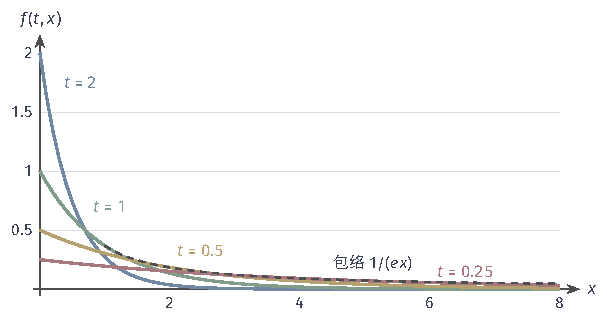
\includegraphics[width=102.807mm]{figures/02-abstract-mathematics/01-metric-and-measure/tikz/c3-parameter-continuity/figure.pdf}
\caption{含参积分中质量的逃逸。四条实线是$f(t,x)=te^{-tx}$在$t=2,1,0.5,0.25$时的图像，每条曲线下的面积都是$1$；$t$越小，质量越向右摊开。虚线是包络$\sup_tte^{-tx}=1/(ex)$（在$t=1/x$处取到，画在$x\geq1$部分），它在无穷远处不可积，所以$t=0$附近没有可积控制。}
\label{fig:integ-parameter-continuity}
\end{figure}

\subsection{积分号下求导}
\label{sec:integ-differentiation-under-integral}

\paragraph{求导定理}
现在设参数取值于开区间$T\subseteq\mathbb R$。$F$在$t$处的差商是$\int\bigl(f(x,t+h)-f(x,t)\bigr)/h\,\mathrm d\mu$，被积函数在$h\to0$时趋于$\partial_tf(x,t)$。要把极限移进积分号，同样需要给差商一个共同的可积上界；由中值定理，差商的大小由导数在参数区间上的大小控制。

\begin{theorem}[积分号下求导]
\label{thm:integ-differentiation-under-integral}
设$T\subseteq\mathbb R$是开区间，$f:X\times T\to\mathbb R$满足：
\begin{enumerate}
 \item 存在$t_0\in T$，使$f(\cdot,t_0)$可积；
 \item 存在零测集$N$，使对每个$x\notin N$，$t\mapsto f(x,t)$在$T$上可微；
 \item 存在可积函数$g\geq0$，使对每个$x\notin N$与每个$t\in T$，$\lvert\partial_tf(x,t)\rvert\leq g(x)$。
\end{enumerate}
则对每个$t\in T$，$f(\cdot,t)$可积，$F(t)=\int_Xf(x,t)\,\mathrm d\mu(x)$在$T$上可微，并且
\[
 F'(t)=\int_X\partial_tf(x,t)\,\mathrm d\mu(x).
\]
复值函数对实部与虚部分别应用即可。
\end{theorem}

\begin{proof}
对$x\notin N$，由中值定理，$\lvert f(x,t)-f(x,s)\rvert\leq g(x)\lvert t-s\rvert$对$s,t\in T$成立。取$s=t_0$，得$\lvert f(x,t)\rvert\leq\lvert f(x,t_0)\rvert+\lvert t-t_0\rvert g(x)$，右边可积，所以每个$f(\cdot,t)$可积。

固定$t\in T$，任取$h_n\to0$且$t+h_n\in T$，$h_n\neq0$。差商$q_n(x)=\bigl(f(x,t+h_n)-f(x,t)\bigr)/h_n$是可测函数，在$N$外收敛到$\partial_tf(x,t)$，所以$\partial_tf(\cdot,t)$在$N$外是可测函数列的极限，可测。由中值定理，$\lvert q_n(x)\rvert\leq g(x)$。由支配收敛定理与线性性，
\[
 \frac{F(t+h_n)-F(t)}{h_n}=\int_Xq_n\,\mathrm d\mu\to\int_X\partial_tf(x,t)\,\mathrm d\mu .
\]
对一切$h_n\to0$都成立，所以$F$在$t$处可微且导数如定理所述。
\end{proof}

导数的控制条件只需在一个参数区间内成立。若条件只在每个$t$附近的某个子区间上成立，把定理用于这些子区间，同样得到$F$在整个$T$上可微。

\begin{example}[逐阶求导]
\label{ex:integ-gamma-derivatives}
对$t>0$，$F(t)=\int_0^\infty e^{-tx}\,\mathrm dx=1/t$。固定$t_0>0$，在$T=(t_0,\infty)$上，$\lvert\partial_te^{-tx}\rvert=xe^{-tx}\leq xe^{-t_0x}$，右边在$[0,\infty)$上可积。由定理，$-\int_0^\infty xe^{-tx}\,\mathrm dx=F'(t)=-1/t^2$。同样的控制$x^ne^{-t_0x}$允许继续求导，归纳得$\int_0^\infty x^ne^{-tx}\,\mathrm dx=n!/t^{n+1}$；取$t=1$即$\int_0^\infty x^ne^{-x}\,\mathrm dx=n!$。由于$t_0>0$任意，结论对一切$t>0$成立；而在$t=0$附近控制失效，$F$本身也在那里趋于无穷。
\end{example}

\paragraph{偏导数逐点存在不等于可以交换}
定理的第3条不能省去。在$[0,\infty)$上取$f(x,t)=t^3e^{-t^2x}$，$t\in\mathbb R$。对$t\neq0$，$F(t)=t^3\cdot t^{-2}=t$；又$F(0)=0$，所以$F(t)=t$，$F'(0)=1$。另一方面，对每个$x\geq0$，
\[
 \partial_tf(x,0)=\lim_{t\to0}\frac{t^3e^{-t^2x}}t=0,
\]
于是$\int_0^\infty\partial_tf(x,0)\,\mathrm dx=0\neq1$。偏导数在每一点都存在，交换却失败了。原因是$\partial_tf(x,t)=(3t^2-2t^4x)e^{-t^2x}$在$t^2=1/x$处等于$1/(ex)$，所以在$0$的任何参数邻域内，它的上包络不小于一个在无穷远处不可积的函数；控制条件必须覆盖参数邻域，只在$t=0$处检查导数是不够的。

\subsection{变动区域上的积分}
\label{sec:integ-moving-domain}

\paragraph{变限的一元积分}
当积分区域也随参数移动时，$F(t)$的变化来自两部分：区域内部的被积函数在变，边界又新添或移除了一部分区域。先看一元的变限积分$F(t)=\int_{a(t)}^{b(t)}f(x,t)\,\mathrm dx$。

\begin{theorem}[变限积分的求导]
\label{thm:integ-variable-limits}
设$J=[\alpha,\beta]$，$T\subseteq\mathbb R$是开区间，$a,b:T\to J$可微。设$f:J\times T\to\mathbb R$连续，$\partial_tf$在$J\times T$上处处存在，并存在可积函数$g\geq0$使$\lvert\partial_tf(x,t)\rvert\leq g(x)$对一切$x\in J$、$t\in T$成立。则$F(t)=\int_{a(t)}^{b(t)}f(x,t)\,\mathrm dx$在$T$上可微，且
\[
 F'(t)=\int_{a(t)}^{b(t)}\partial_tf(x,t)\,\mathrm dx+f\bigl(b(t),t\bigr)b'(t)-f\bigl(a(t),t\bigr)a'(t).
\]
\end{theorem}

\begin{proof}
固定$t$，取$h\neq0$且$t+h\in T$，记$a=a(t)$、$a_h=a(t+h)$，$b,b_h$同理。把增量拆成三部分：
\begin{equation*}
\begin{aligned}
 F(t+h)-F(t)={}&\int_a^b\bigl(f(x,t+h)-f(x,t)\bigr)\mathrm dx\\
 &+\int_b^{b_h}f(x,t+h)\,\mathrm dx-\int_a^{a_h}f(x,t+h)\,\mathrm dx .
\end{aligned}
\end{equation*}
第一项除以$h$后，由定理~\ref{thm:integ-differentiation-under-integral}的论证（差商由$g$控制，支配收敛）趋于$\int_a^b\partial_tf(x,t)\,\mathrm dx$。

第二项来自上端点的移动。$f$在$(b,t)$处连续，对$\varepsilon>0$，当$h$足够小时，$b_h$与$b$之间的每个$x$都满足$\lvert f(x,t+h)-f(b,t)\rvert<\varepsilon$。于是
\[
 \Bigl\lvert\frac1h\int_b^{b_h}f(x,t+h)\,\mathrm dx-\frac{b_h-b}hf(b,t)\Bigr\rvert\leq\varepsilon\Bigl\lvert\frac{b_h-b}h\Bigr\rvert,
\]
而$(b_h-b)/h\to b'(t)$，所以第二项除以$h$趋于$f(b,t)b'(t)$。第三项同理趋于$f(a,t)a'(t)$。
\end{proof}

两个边界项符号相反：上端向右移动增加积分区域，下端向右移动减少积分区域。例如$F(t)=\int_0^txt\,\mathrm dx=t^3/2$，直接求导得$3t^2/2$；按定理计算，内部变化贡献$\int_0^tx\,\mathrm dx=t^2/2$，上端移动贡献$f(t,t)\cdot1=t^2$，合计$3t^2/2$，两者一致。与卷二在连续可微条件下的同一公式相比，这里只要求被积函数连续、参数导数有可积控制，内部项的交换完全由支配收敛负责；连续性只在边界点上用于读出新添部分的高度。

\paragraph{有参数的多元区域}
在$\mathbb R^d$中，区域的移动不能只用两个端点描述，需要把区域参数化。设$\Omega_0\subseteq\mathbb R^d$是开集，对每个$t\in T$，$\Phi_t:\Omega_0\to\Omega_t$是连续可微的双射，逆映射也连续可微，记$J_t(y)=\lvert\det D\Phi_t(y)\rvert$。由卷二的积分换元公式（可参考\BookChapterRef{chap:region-integrals}{卷二第21章“区域积分”}），
\[
 F(t)=\int_{\Omega_t}f(x,t)\,\mathrm dx=\int_{\Omega_0}f\bigl(\Phi_t(y),t\bigr)J_t(y)\,\mathrm dy,
\]
右端是固定区域上的积分。

于是变动区域的问题化为固定区域上的含参积分：只要对几乎每个$y$，映射$t\mapsto f(\Phi_t(y),t)J_t(y)$可微，并且这个参数导数在$T$上有与$t$无关的可积上界，就可以用定理~\ref{thm:integ-differentiation-under-integral}在积分号下求导。这里有两类条件：边界的移动由参数化$\Phi_t$的光滑性描述，被积函数的变化由支配条件控制，二者都要在使用前核对。一元情形取$\Phi_t(y)=a(t)+y(b(t)-a(t))$，$\Omega_0=(0,1)$，得到的正是上面的公式。

在$\Phi$足够光滑时，把导数写回$\Omega_t$上，并用散度定理把与区域移动有关的部分改写成边界上的通量，可以得到边界项的多元形式：它沿整个边界累计被积函数乘以边界的法向移动速度。这一改写需要边界的光滑性与散度定理，这里不展开推导。
